% Candidate figure snippets only. Do not include this file directly.

\begin{figure}[t]
\centering
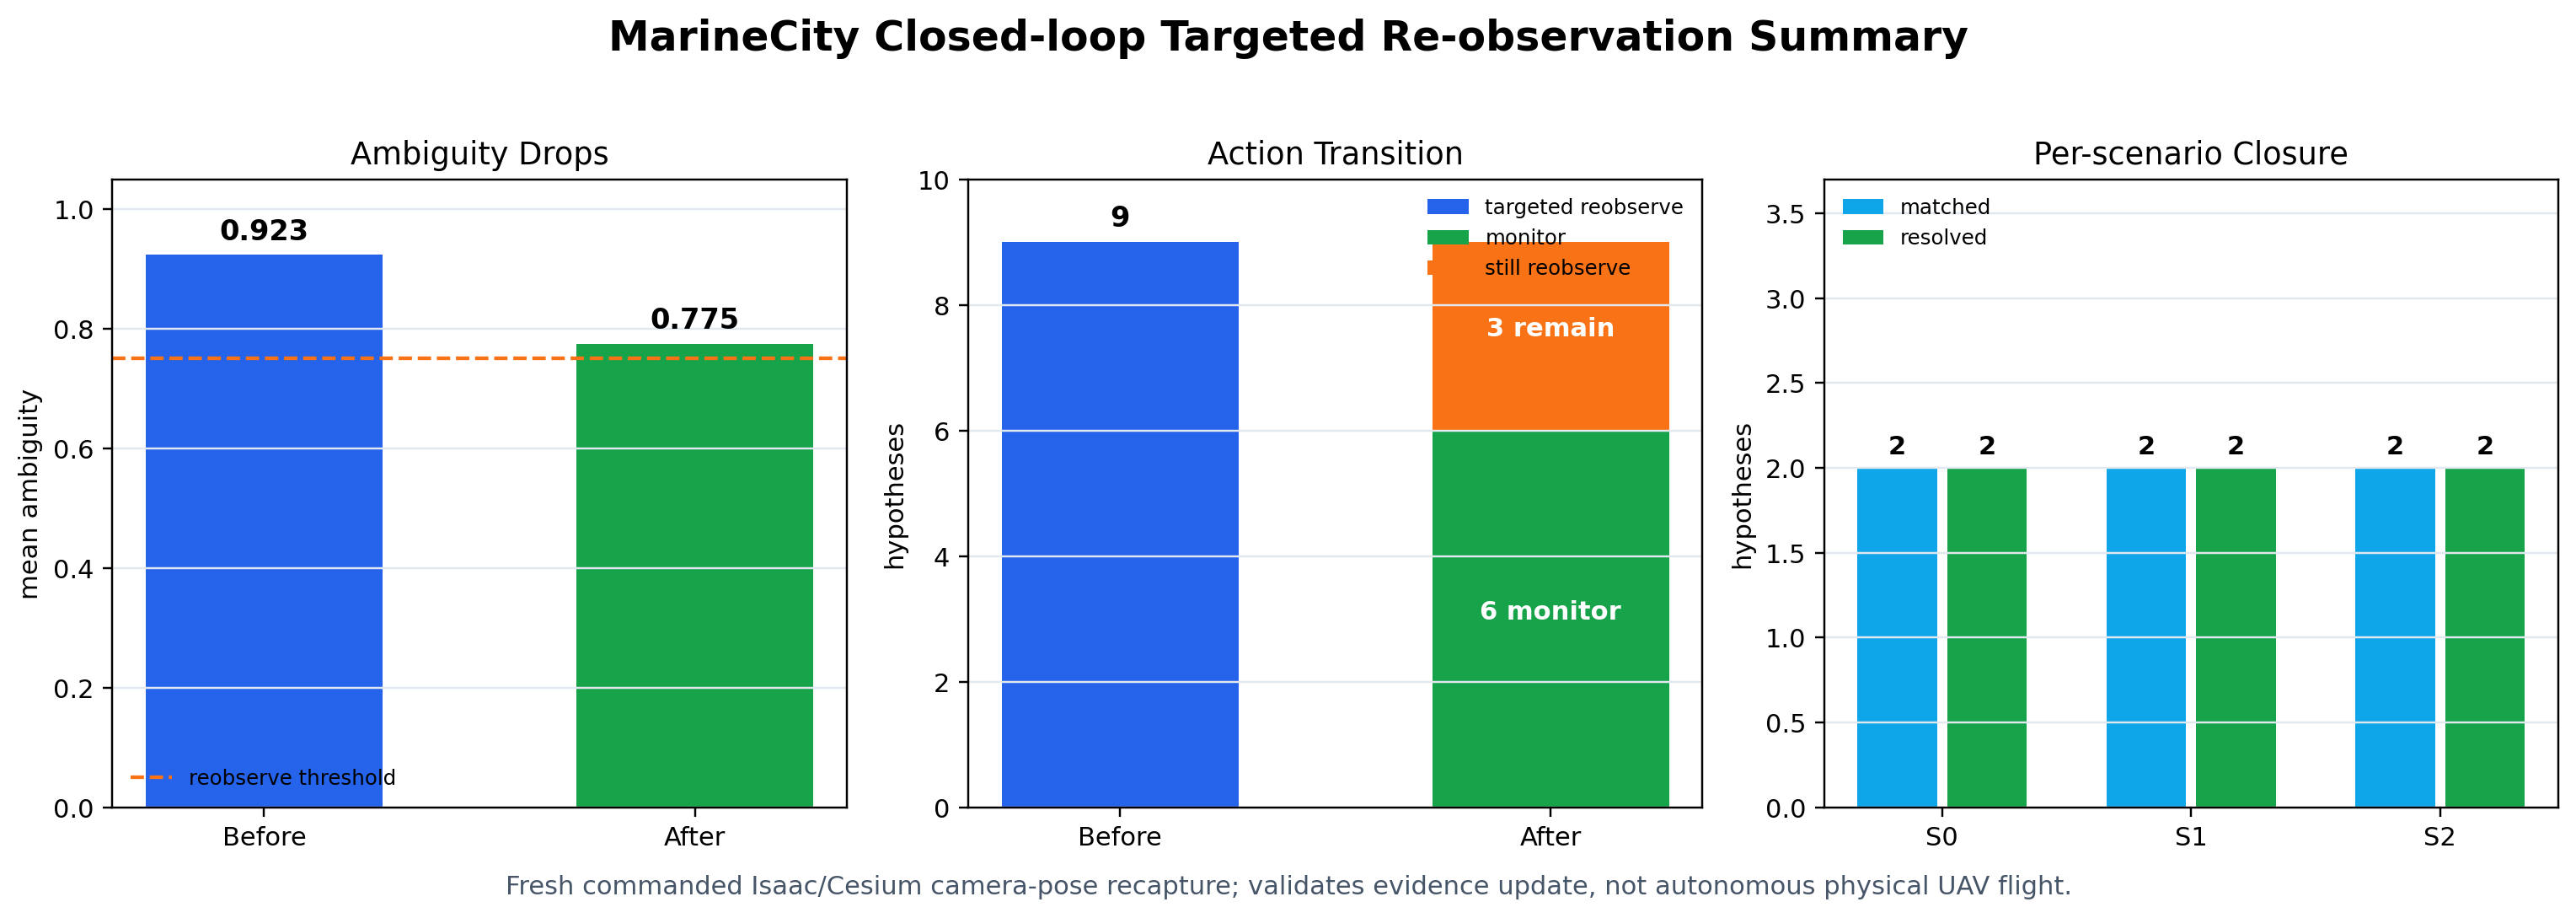
\includegraphics[width=0.95\linewidth]{revision_guidance/closed_loop_reobservation_20260703/figures/closed_loop_summary_card.png}
\caption{Summary of the MarineCity targeted re-observation evidence update.
Fresh commanded Isaac/Cesium camera-pose recapture provides matching evidence
for six of nine routed hypotheses, moving them from targeted re-observation to
monitor while leaving three hypotheses queued for further evidence.}
\label{fig:candidate_closed_loop_summary_card}
\end{figure}

\begin{figure}[t]
\centering
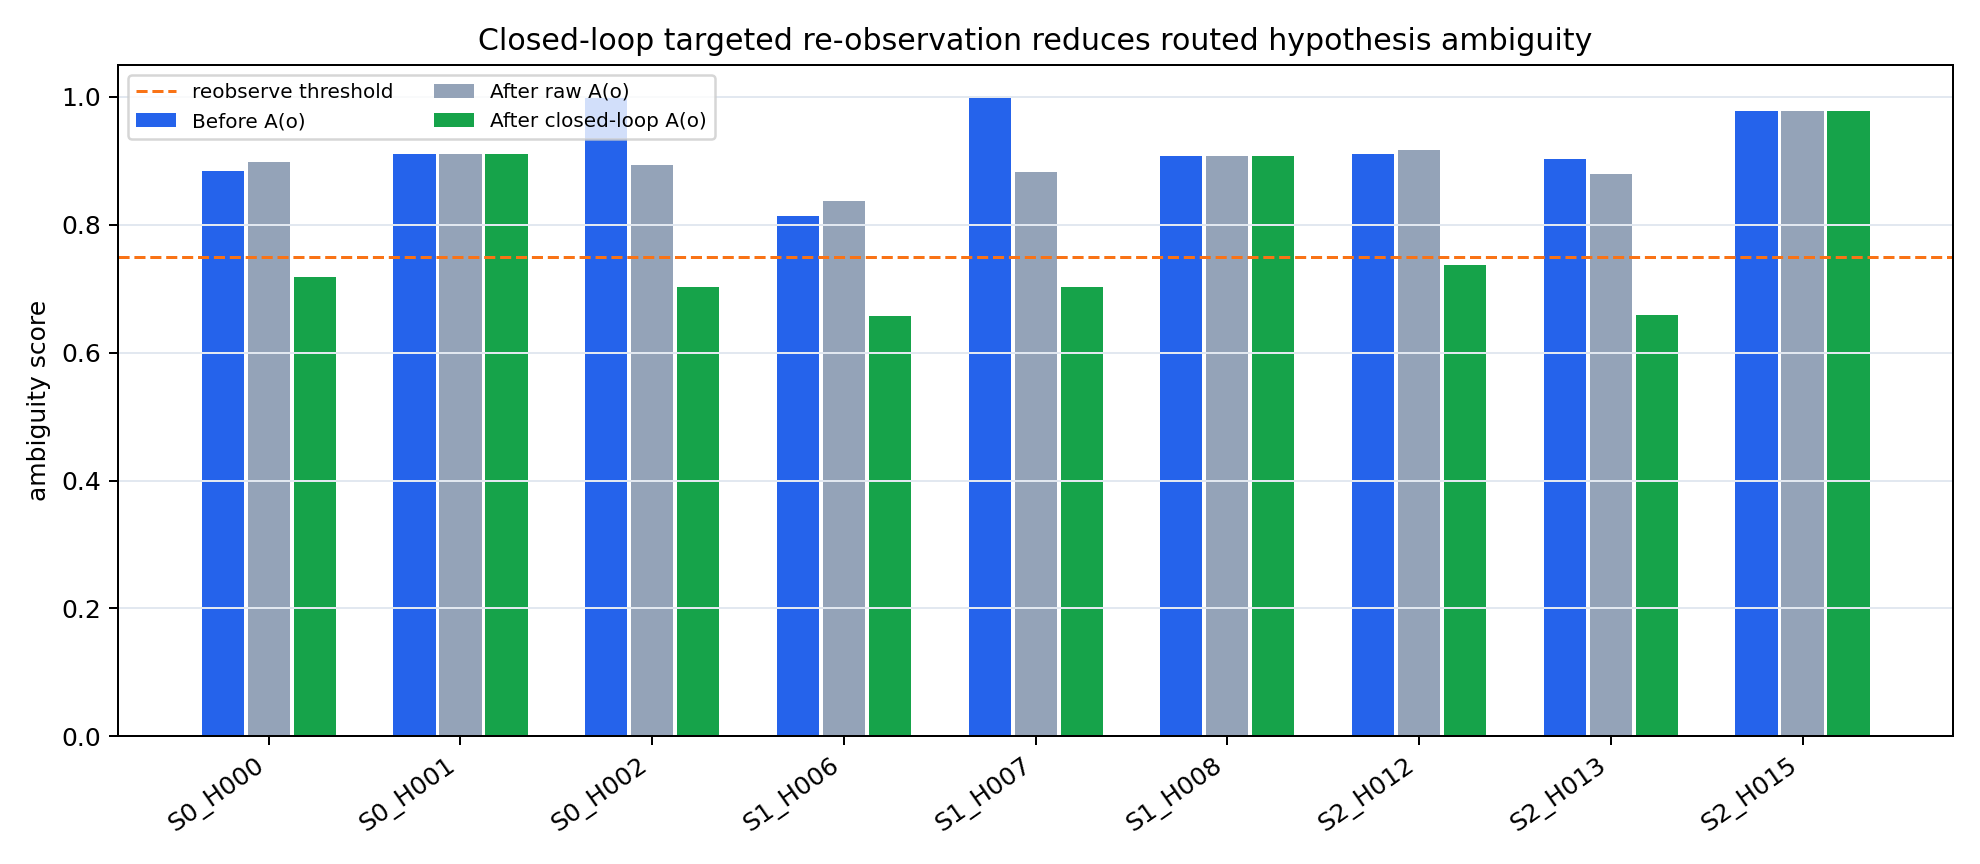
\includegraphics[width=0.92\linewidth]{revision_guidance/closed_loop_reobservation_20260703/figures/closed_loop_ambiguity_before_after.png}
\caption{Closed-loop re-observation evidence update over the nine MarineCity
hypotheses routed to targeted re-observation. Fresh commanded Isaac/Cesium
recapture evidence reduces ambiguity for six hypotheses, while hypotheses
without matching same-class follow-up evidence remain in the re-observation
queue.}
\label{fig:candidate_closed_loop_ambiguity_before_after}
\end{figure}

\begin{figure*}[t]
\centering
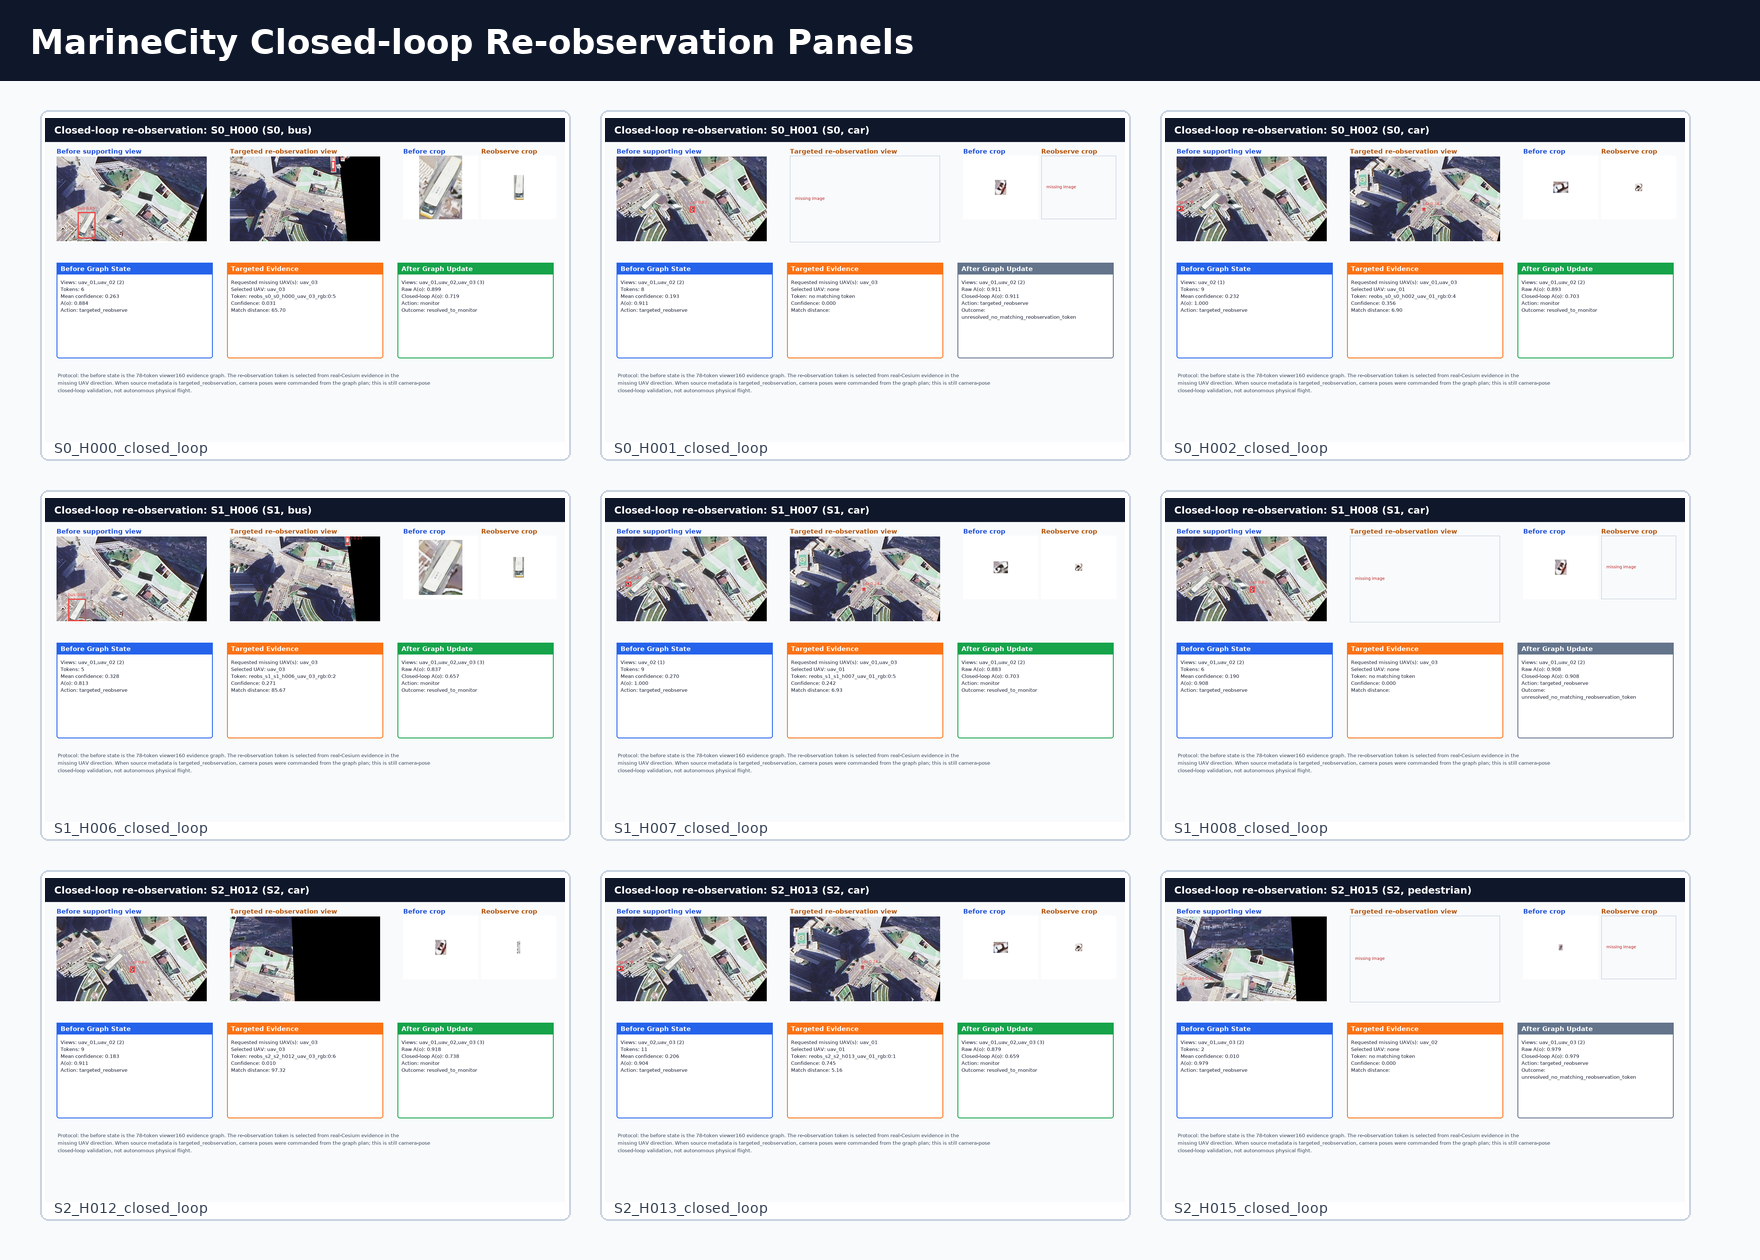
\includegraphics[width=0.98\textwidth]{revision_guidance/closed_loop_reobservation_20260703/figures/closed_loop_contact_sheet.png}
\caption{Closed-loop re-observation contact sheet. Each panel shows a routed
hypothesis, the matched fresh re-observation evidence when available, and the
recomputed graph action. Six hypotheses move from targeted re-observation to
monitor after evidence completion; three remain queued because no matching
same-class recapture token is available.}
\label{fig:candidate_closed_loop_contact_sheet}
\end{figure*}
